\documentclass[14pt, twocolumn]{article}
\usepackage[margin=0.5in]{geometry} 
\usepackage{amsmath,amsthm,amssymb}
\usepackage{graphicx}
\usepackage{colortbl}
\usepackage{xcolor}
\usepackage{multirow}
\pagenumbering{gobble}

% Makes stuff clickable
% \usepackage{hyperref}
% \hypersetup{
%     colorlinks,
%     citecolor=black,
%     filecolor=black,
%     linkcolor=black,
%     urlcolor=black
% }

\title{FREEZE!: Pretrained Language Models as Frozen Feature Extractors for Semantic Tasks}
\author{
    Hayden McDonald\\hayden\_mcdonald@brown.edu \and 
    Nicholas Marsano\\nicholas\_marsano@brown.edu\and 
    Oliver McLaughlin\\oliver\_mclaughlin@brown.edu
}

\begin{document}

\maketitle

% Title: Summarizes the main idea of your project.
% Who: Names and logins of all your group members.

\setcounter{tocdepth}{4}
\setcounter{secnumdepth}{4}
\tableofcontents
\newpage

\section{Introduction}
% Introduction: What problem are you trying to solve and why?
%     Detail how you arrived at this topic and what motivated you.
%     What kind of problem is this? Classification? Regression? Structured prediction? Reinforcement Learning? Unsupervised Learning? etc.
Our project is an investigation into a few related areas. In short, we wanted to see if we could develop an architecture that could take the intermediate activations of a pre-trained decoder-only large language model (Henceforth LLM) and use them to do text-embedding tasks. We chose semantic sentence similarity (STS) as our primary focus and motivation because of its simplicity. This task involves training a model to rate the semantic similarity of a pair of sentences. Importantly, in contrast to most other work using LLMs for text embedding, we are \textit{not} fine-tuning the model. We are simply taking a subset of the intermediate activations and treating them as a kind of \textit{"feature extracted"} (frozen) representation.\\\\
We chose this idea for several reasons.
\begin{enumerate}
    \item Our original motivational question was: \textit{"Do ‘similar’ prompts (to human readers) have ‘similar’ (under some metric) representations to a given language model?"}. By training a sentence-similarity model on LLM activations, we believed we could make progress on answering this question by \textit{learning} a transformation of the activations that correlates to semantic similarity.

    \item \textit{If} we could train a small model to interpret a given LLM's activations and produce a useful text embedding (or set of embeddings) from them, we could skip costly fine-tuning and simply pre-train and fine-tune the small "interpreter" model. Pretrained small LLMs are cheap to do forward passes on and very plentiful, so if we could \textit{just} use the intermediate activations and not have to do backward passes we could get a lot of functionality for very little compute.
    
    \item We also wanted to investigate the question: \textit{Do multiple intermediate activations perform better than just the last?} Typically when doing finetuning or transfer learning you remove the classifier end and use the last intermediate representation as your "feature extracted representation". We wanted to see if there was any performance benefit in using \textit{multiple layer's} worth of representation. This is clearly the case in the finetuning setting \cite{tang2024poolingattentioneffectivedesigns} but it's unclear if it will work here.
    
    \item From an interpretability standpoint, most distance or similarity measures (E.g cosine similarity) do not correlate strongly with \textit{human ideas} of similarity (Figure \ref{fig:raw-corr}). By training a similarity learner on LLM activations, grounded in human ideas of similarity, we hoped to produce a more interpretable measure of similarity for LLM activations.
    
    \item There just isn't that much work on this particular topic. For this task you'd typically finetune the LLM using LoRA \cite{hu2021loralowrankadaptationlarge} or simply just use an existing text embedding model. We hoped to discover interesting properties and learn a lot about what it's like to try and \textit{"disentangle"} an LLM's intermediate activations into something useful by pursuing this project. \footnote{There was only one paper we could find doing a similar setup -- extracing latents from an LLM and applying them to a task -- but it is very low quality and does not reveal many of the important details \cite{gpt2malware}. There are many papers \textit{like} this one (\cite{lu2021pretrainedtransformersuniversalcomputation} comes to mind) but almost none completely freeze the entire model and "start from scratch" as we did here.} We're not really interested in \textit{what} information is \text{where}, we just want to see \textit{if it's useable} for a simple task like STS.
    
\end{enumerate}
We chose \verb|gpt2-medium| (355M parameters) as our \textit{"base model"} for study because Oliver was familiar with its architecture and it readily fit onto all of our GPUs. We also did minor experiments on \verb|qwen2-0.5B| (391M parameters). Moreover we chose \verb|gpt2-medium| because of its very low quality text generation ability. It was not at all a priori obvious to us that its representations would be fit for this task.

\begin{figure}[!htb]
    \centering
    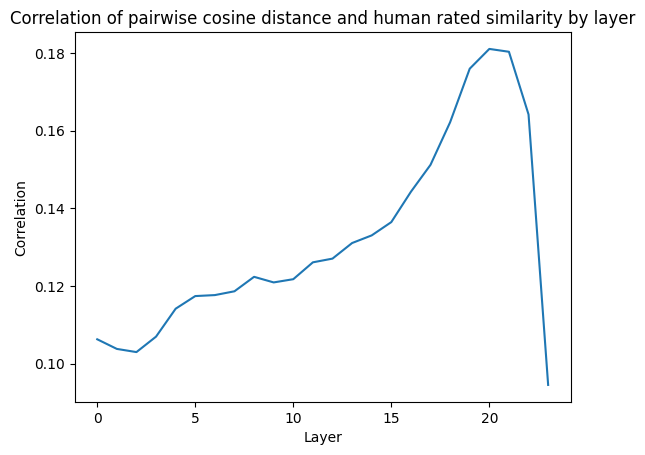
\includegraphics[width=1\linewidth]{raw_cosine_sim.png}
    \caption{\textbf{The problem we are ultimately trying to solve}. Layerwise average correlation between gpt1-medium's embeddings and their cosine similarity vs. human similarity score for the STS training pairs}
    \label{fig:raw-corr}
\end{figure}

\subsection{Problem Setup} \label{Setup}
Figure \ref{fig:raw-corr} was our "starting point". This figure depicts the correlation between two important quantities for our investigation:
\begin{enumerate}
    \item The cosine similarity of two sentences' latent representations (See \ref{latent} for more information on this representation)
    \item A human rated similarity score for those same two sentences (See \ref{STS-section})
\end{enumerate}
For each layer we computed the mean correlation between these two quantities for more than five thousand sentence pairs. This is essentially the problem we are trying to solve -- \textit{How can we transform these latent representations into something useable for semantic text similarity?}

\section{Related Work}
% Related Work: Are you aware of any, or is there any prior work that you drew on to do your project?
%     Please read and briefly summarize (no more than one paragraph) at least one paper/article/blog relevant to your project.
Reusing pretrained LLMs for semantic tasks like STS is nothing new. There is extensive literature about finetuning and retraining
these models for a variety of new tasks (CITE ME). Moreover using decoder-only models for embedding tasks is common, with works like
SGPT (CITE ME), LLM2VEC, etc.\\\\
It is well known that GPT-2 produces incredibly low quality embeddings (CITE ME. https://arxiv.org/pdf/1909.00512)

\section{Data}
We have three major datasets that we used for both pretraining and supervised STS training.
\begin{enumerate}
    \item STSB \cite{STS} -- A standard sentence similarity benchmark with associated training and test sets.
    \item GenericsKB \cite{bhakthavatsalam2020genericskbknowledgebasegeneric} -- A 'generic sentence' dataset of which we used twenty-thousand examples.
    \item SNLI \cite{snli} -- An inference relation dataset. Used in a pretraining experiment and in Sentence-BERT \cite{reimers2019sentencebertsentenceembeddingsusing}
\end{enumerate}

\subsection{Semantic Text Similarity Benchmark (STSB)} \label{STS-section}
The main task we targeted was STSB \cite{STS}, which is a benchmark for semantic text similarity. It's comprised of pairs of sentences and a human-rated "similarity score". For example:
$$
(\text{s1='A plane is taking off.'}, \text{s2='An air plane is taking off.'}, \text{sim}=1.0)
$$
The performance metrics for STS are typically Spearman's rank correlation coefficient and normal Pearson correlation between the predicted similarities of pairs of sentences and the human rated similarities. State of the art for this task is around \verb|90 - 92%| in both spearman and pearson according to the MTEB leaderboard \cite{muennighoff2022mteb}.

\subsection{Data Collection and Pipeline} \label{latent}
Our data pipeline is fairly simple. We're treating \verb|gpt2-medium| as a feature extractor, so for each piece of text for any task, we simply pass that text through the model and extract a latent representation from the intermediate activations at each layer. We chose to take the \textit{last token at each layer, after the residual connection} (Henceforth called a \textit{latent}). This strategy is not original and is fairly standard in the \textit{fine tuning} literature \cite{LLMEmbed}. We expected it to do fine for our task given that \verb|gpt2-medium| uses causal attention, even though we're not fine tuning. This gives us, for each sentence, twenty-four \verb|1024| dimensional vectors (\verb|n_layers x d_model|). One of the main challenges we wanted to overcome by taking this project on was finding a sensible way to \textit{actually use} such a high volume and dimensionality of data.
% Data: What data are you using (if any)?

%     If you’re using a standard dataset (e.g. MNIST), you can just mention that briefly. Otherwise, say something more about where your data come from (especially if there’s anything interesting about how you will gather it).
%     How big is it? What kind of preprocessing was required?

\section{Methodology}
% Methodology: What is the architecture of your model?
%     How are you training the model?
%     Justify your design. Also note some things you tried that may or may not have worked.
\subsection{Training and Loss function} \label{Loss} \label{Training}
Our general training scheme was the following:
\begin{enumerate}
    \item Pass whatever example sentence for the current task through \verb|gpt2-medium|
    \item Extract the latents (Described in Section \ref{latent}) from each layer. We take these latents and completely decouple them from the base model. They are effectively just a set of vector representations of the input. No gradient is passed back through \verb|gpt2-medium|
    \item Pass those latents into our model.
\end{enumerate}
Our loss function for supervised STS training departs from the traditional mean squared-error (MSE) in that we only try and minimize the \text{variance of the residuals}, instead of the traditional variance \text{and} bias which are both minimized when using MSE.

\subsection{Architecture}
Our architecture was decided through a series of experiments and trial and error. We tried to only make architectural decisions which were, in some way, \textit{principled} -- I.e. we had a decent reason for making that particular change.

\subsection{First iteration}
Our first architecture was incredibly simple -- Just take the layerwise cosine similarities described in Section \ref {Setup} and pass them through an MLP to do basic weighting and statistical correlation. We felt this was reasonable because although the individual correlations were quite weak, it wasn't clear to us that each layer was correlating \textit{to the same content}. In the same way that many weak models can be combined to create a strong one, we figured that a simple MLP would be able to decipher some of the more complicated relationships, even just through the layerwise similarities. This model was quite simple, just a one layer mlp that took the twenty-four layerwise cosine similarities from \verb|gpt2-medium|'s respective latents and outputted a sigmoided single scalar. This was trained using the scheme described in Section \ref{Training}. This model significantly improved upon baseline, giving us a test set pearson correlation of \verb|39.2%| and spearman of \verb|42.06%| ($p<< 0.001$)

\subsection{Layerwise Siamese Networks}
After the previous architectural experiment, we figured that we were probably bottlenecked by the representation of our base model, necessitating a transformation. Inspired by prior work on Siamese networks for semantic tasks \cite{reimers2019sentencebertsentenceembeddingsusing}, we decided to modify our architecture by applying siamese networks to each layer, computing the cosine similarities of \text{those} representations, and then finally passing those cosine similarities into a weighting/pattern matching MLP as described above. The intuition here is that each layer probably contains meaningfully different and useful information, as evidence by weighted cosine doing better than any particular layer. So, if we learn a nonlinear transformation of each layer's particular space through supervised STS training, we might be able to extract a better representation for this task and have overall better downstream performance.\\\\
This architecture achieved a \text{significant} performance increase, moving our pearson and spearman on the test set to \verb|71.63%| and \verb|69.72| ($p << 0.001$) respectively.

\subsection{Autoencoder pretraining and the final model}
We then realized that although this architecture was traning quite well, it was likely the case that inputs which were significantly different from those in the input distribution would likely not be well represented by our siamese networks. This then inspired us to change our training strategy. Our current strategy \text{coupled} our representation learning and our supervised STS learning. That is, the model had to both learn a good representation of the input whilst also learning how to orient examples spatially to reflect semantic similarity. We then decided to break this up by first training a set of layerwise autoencoders over twenty-thousand "generic" sentences from the GenericsKB \cite{bhakthavatsalam2020genericskbknowledgebasegeneric} dataset. These senteces were similar in length and complexity to the STS training set that we felt it was an appropriate 'pretraining' dataset. We trained the autoencoders to reconstruct each layer's latent for each sentence (I.e. twenty-four autoencoders, each trying to reconstruct their respective layer's latent). We then did this pretraining and took the encoder part of each autoencoder and treated it as our new siamese network. Each autoencoder had a bottleneck of $256$ hidden units.\\\\
Immediately, our results were \textit{indistinguishable} from the results of the previous section. We then produced Figure (PUT FIGURE) and realized that the layerwise losses for each autoencoder increased exponentially as the layers went on. This inspired us to, among many other things, widen the bottleneck of the last twelve autoencoders from $256$ to $512$. This then finally showed a performance increase to \verb|75.36%| pearson and \verb|73.21%| spearman. Our final change was to incorperate the loss function switch described in Section \ref{Loss}, which brought us to a final pearson and spearman correlation of:
\begin{align*}
    &\text{Pearson} = 76.86\%\\
    &\text{Spearman} = 75.03\%\;,\; p << 0.001
\end{align*}
Moreover, this architecture actually ended up with more than $600,000$ fewer parameters when compared to our previous best model.

\subsection{Experiments that failed}


% Our loss function has evolved significantly since the beginning. We plotted the distribution of our residuals and noticed
% the spread could be tightened. Since this is a correlative task, we don't care about bias, just variance. So instead of doing MSE
% we just optimize to minimize the variance of the residuals directly
% $$
% \mathcal{L}(\theta) = \log(\text{Var}(y - \hat{y}))
% $$
% Where the added log improved stability

\section{Results}
\subsection{Requirements for success}
Our main notion of success was performance on the STSB \cite{STS} benchmark as described in Section \ref{STS-section}. Pearson/spearman correlation are both reasonable measures of success on this task because they measure how consistent your model is with human-rated similarity notions, regardless of scale or center. State of the art on this task is \verb|90-92%| for both Spearman and Pearson correlation as of the writing of this document \cite{muennighoff2022mteb}. Our goal was to achieve at least \verb|60%| pearson correlation. We really did not have strong reasoning for why this might be a reasonable goal but preliminary results showed that at least \verb|40%| was possible so we decided that \verb|60%| was a reasonable stretch goal

\subsection{Final Results}
We achieved a Pearson correlation on STSB's test set of \verb|76.86%| and a Spearman correlation of \verb|75.3%| with a p-value of significantly less than \verb|0.0001|.
% Results: What constitutes “success?”
%     What experiments did you run?
%     For most of our assignments, we have looked at the accuracy of the model. Does the notion of “accuracy” apply for your project, or is some other metric more appropriate?
%     Explain how you assess your model's performance and justify why it is a reasonable measurement.

\section{Ethics}
% Ethics: Choose 2 of the following bullet points to discuss; not all questions will be relevant to all projects so try to pick questions where there’s interesting engagement with your project. (Remember that there’s not necessarily an ethical/unethical binary; rather, we want to encourage you to think critically about your problem setup.)
%     What broader societal issues are relevant to your chosen problem space?
%     Why is Deep Learning a good approach to this problem?
%     What is your dataset? Are there any concerns about how it was collected, or labeled? Is it representative? What kind of underlying historical or societal biases might it contain?
%     Who are the major “stakeholders” in this problem, and what are the consequences of mistakes made by your algorithm?
%     How are you planning to quantify or measure error or success? What implications does your quantification have?
%     Add your own: if there is an issue about your algorithm you would like to discuss or explain further, feel free to do so.

\section{Reflection}
% Reflection: please address the following questions (along with other thoughts you have about the project, if any):
%     How do you feel your project ultimately turned out? How did you do relative to your base/target/stretch goals?
%     Did your model work out the way you expected it to?
%     How did your approach change over time? What kind of pivots did you make, if any? Would you have done differently if you could do your project over again?
%     What do you think you can further improve on if you had more time?
%     What are your biggest takeaways from this project/what did you learn?

One big takeaway from this project is that as gigantic open source LLMs become more pevalent, it might be possible to chop off most of their layers and train little "interpreter" modules as we did here to leverage the incredibly rich and complex learned represenations at a fraction of the cost and computation time.

\section{Division of Labor}
% Division of labor: Briefly outline who will be responsible for which part(s) of the project.
\begin{itemize}
    \item \textit{Hayden.}
    \item \textit{Nick.} 
    \item \textit{Oliver.} 
\end{itemize}

\newpage
\section{Appendix: \textit{STSB} dataset leakage}

%% --------------------------------------------------------------
%%                         Start here
%% --------------------------------------------------------------
%% \hline
% \section{Check-in Highlights}
% \subsection{Introduction}
% Our project is essentially trying to figure out if using a small LLM like \verb|gpt2-medium| as a feature extractor (Frozen, we don't fine-tune it. Exactly like \verb|CLIP| in homework four) is a viable option for a simple task like semantic text similarity (STS) \cite{STS}. At its face, taking basically any of GPT-2's activations (E.g. last token, last layer) produces incredibly low quality embeddings for STS (Less than $20\%$ pearson correlation. See figure \ref{fig:raw-corr}). Although using LLMs for text embedding is increasingly common \cite{LLM2Vec} \cite{NVEmbed} \cite{RepImprovesLLM} \cite{LLMEmbed}, there are very few papers who \textit{do not fine-tune or modify} the original LLM. Our goal was to find a decent architecture that can make sense of \verb|gpt2-medium|'s embeddings and produce a viable STS model. STS performance is measured by the pearson correlation between a model's similarity judgment for a set of sentence pairs and a set of human similarity scores. State of the art on this task is \verb|90-93%| correlation. The data used to train our model are the twenty-four (\verb|gpt2-medium| has twenty-four layers) final tokens at each layer after the final residual connection has been added. This is a standard latent \footnote{We refer to this "final token at each layer after the final residual connection" as the layer's "latent" for the remainder of this report. We use the term "latent" and "activation" interchangeably.} to extract when finetuning LLMs \cite{LLMEmbed}, particularly for decoder-only models like GPT-2 where the final token has attended to the entire sequence. We felt it was reasonable enough choice even if we're not finetuning. These are extracted from \verb|gpt2-medium| after a given sentence is passed through and can be understood as twenty-four "embeddings" produced by the LLM for a particular sentence.

% \subsection{Insights}
% The most interesting thing we can share so far is our supervised performance on STSB (STS Benchmark) on which we achieve \verb|75.36%| pearson correlation. Although not state of the art, we're incredibly happy with this result considering our approach is incredibly experimental and we got this result with (comparatively) very little computational resources.\\\\
% The model we used to achieve this is a modified layerwise siamese network (As in we take a latent vector at each layer of \verb|gpt2-medium| and feed it into a designated siamese network) with an unsupervised pretraining step prior to supervised STS training (See the \textit{"Architecture"} section below for more details and clarifications). Our score is more than \textit{triple} the performance of the raw embeddings produced natively by \verb|gpt2-medium| (Figure \ref{fig:raw-corr}). We also found strong empirical evidence for the hypothesis that later layers in transformer models store meaningfully more "information" (In the information theoretic sense) than earlier layers (See the \textit{"Accidental reproduction"} section below for more information) which directly influenced changes to our pretraining approach, breaking our previous correlation record of \verb|68%|.

% \subsection{Challenges}
% We've faced a number of challenges, most of them related to training and regularizing our model. We've found this architecture and dataset to be highly resistant to hyperparameter changes and vulnerable to overfitting. Throughout many, many hyperparameter experiments we found no benefit from added dropout, learning rate changes, deeper siamese networks, among other changes (See the \textit{"Hyperparameter woes"} section below for more details). Our model also produces low quality unsupervised embeddings (\verb|~30-40%| pearson correlation), which is likely an artifact of our pretraining approach focusing on compression over preserving semantic relationships. Moreover, we found that more pretraining (\verb|>20k| sentences) actually decreased performance in almost every scenario, while too little pretraining reverted us back to baseline performance, suggesting a surprisingly narrow optimal window for the pretraining phase.

% \subsection{Plan}
% Our immediate focus is on systematic hyperparameter optimization using Optuna. Although our previous hyperparameter experiments were discouraging, we believe a more principled search of the parameter space might reveal configurations we missed, particularly for the autoencoder pretraining phase. We're also working to finalize our supervised performance results and potentially improve them through targeted regularization strategies. The significant gap between our supervised and unsupervised performance (\verb|75.36%| vs \verb|~30-40%|) remains a key area of investigation - we want to better understand if this gap reveals something fundamental about how GPT-2 encodes semantic information or if it's merely an artifact of our training approach. Finally, we're exploring various pooling strategies to produce single-vector embeddings rather than our current layer-wise approach. If successful, this would make our model more generally applicable beyond pure STS tasks and potentially reveal more about how semantic information is distributed across GPT-2's layers.\\\\
% One particularly promising direction we want to explore is replicating the NLI pretraining approach from Sentence-BERT \cite{reimers2019sentencebertsentenceembeddingsusing}. Given that overfitting has been a persistent challenge with our many small independent models, we believe additional pretraining on a structured task like NLI could help build more robust representations before STS fine-tuning. Whether or not it's possible to do a complex causal reasoning task like NLI solely using LLM latents is yet to be seen.

% % No more highlights B)
% \newpage

% \section{Thorough check-in}
% \subsection{Introduction}
% Our project is an investigation into a few related areas. In short, we wanted to see if we could develop an architecture that could take the intermediate activations of a pre-trained decoder-only large language model (Henceforth LLM) and use them to do text-embedding tasks. We chose sentence similarity as our primary focus and motivation because of its simplicity. Importantly, in contrast to most other work using LLMs for text embedding, we are \textit{not} fine-tuning the model. We are simply taking a subset of the intermediate activations and treating them as a kind of \textit{"feature extracted"} (frozen) representation.\\\\
% We chose this idea for several reasons.
% \begin{enumerate}
%     \item Our original motivational question was: \textit{"Do ‘similar’ prompts (to human readers) have ‘similar’ (under some metric) representations to a given language model?"}. By training a sentence-similarity model on LLM activations, we believed we could make progress on answering this question by \textit{learning} a transformation of the activations that correlates to semantic similarity.

%     \item \textit{If} we could train a small model to interpret a given LLM's activations and produce a useful text embedding (or set of embeddings) from them, we could skip costly fine-tuning and simply pre-train and fine-tune the small "interpreter" model. Pretrained small LLMs are cheap to do forward passes on and very plentiful, so if we could \textit{just} use the intermediate activations and not have to do backward passes we could get a lot of functionality for very little compute.

%     \item We also wanted to investigate the question: \textit{Do multiple intermediate activations perform better than just the last?} Typically when doing finetuning or transfer learning you remove the classifier end and use the last intermediate representation as your "feature extracted representation". We wanted to see if there was any performance benefit in using \textit{multiple layer's} worth of representation. This is clearly the case in the finetuning setting \cite{tang2024poolingattentioneffectivedesigns} but it's unclear if it will work here.

%     \item From an interpretability standpoint, most distance or similarity measures (E.g cosine similarity) do not correlate strongly with \textit{human ideas} of similarity (Figure \ref{fig:raw-corr}). By training a similarity learner on LLM activations, grounded in human ideas of similarity, we hoped to produce a more interpretable measure of similarity for LLM activations.
    
%     \item There just isn't that much work on this particular topic. For this task you'd typically finetune the LLM using LoRA \cite{hu2021loralowrankadaptationlarge} or simply just use an existing text embedding model. We hoped to discover interesting properties and learn a lot about what it's like to try and \textit{"disentangle"} an LLM's intermediate activations into something useful by pursuing this project. \footnote{There was only one paper we could find doing a similar setup -- extracing latents from an LLM and applying them to a task -- but it is very low quality and does not reveal many of the important details \cite{gpt2malware}}

% \end{enumerate}
%  We chose \verb|gpt2-medium| (355M parameters) as our \textit{"base model"} for study because Oliver was familiar with its architecture and it readily fit onto all of our GPUs. We also did minor experiments on \verb|qwen2-0.5B| (391M parameters).

% \subsubsection{Training and Performance Metrics}
% We chose to target the STS Benchmark \cite{STS} which is a supervised sentence similarity benchmark comprised of sentence pairs and a human rated similarity score (E.g. \textit{('A plane is taking off.', 'An air plane is taking off.', sim=1)}).\\\\
% We began our investigations by first choosing which intermediate activations from \verb|gpt2-medium| to feed into our model. We chose to take the \textit{last token at each layer, after the residual connection} (Henceforth called a \textit{latent}). This strategy is not original and is fairly standard in the \textit{fine tuning} literature \cite{LLMEmbed}. We expected it to do fine for our task given that \verb|gpt2-medium| uses causal attention, even though we're not fine tuning.\\\\
% This gives us, for each sentence, twenty-four \verb|1024| dimensional vectors (\verb|n_layers x d_model|). One of the main challenges we wanted to overcome by taking this project on was finding a sensible way to \textit{actually use} such a high volume and dimensionality of data.\\\\
% The performance metrics for STS are typically Spearman's rank correlation coefficient and normal Pearson correlation between the predicted similarities of pairs of sentences and the human rated similarities. State of the art for this task is around \verb|90 - 92%| in both spearman and pearson according to the MTEB leaderboard \cite{muennighoff2022mteb}.

% \subsubsection{Architecture}
% \begin{figure}
%     \centering
%     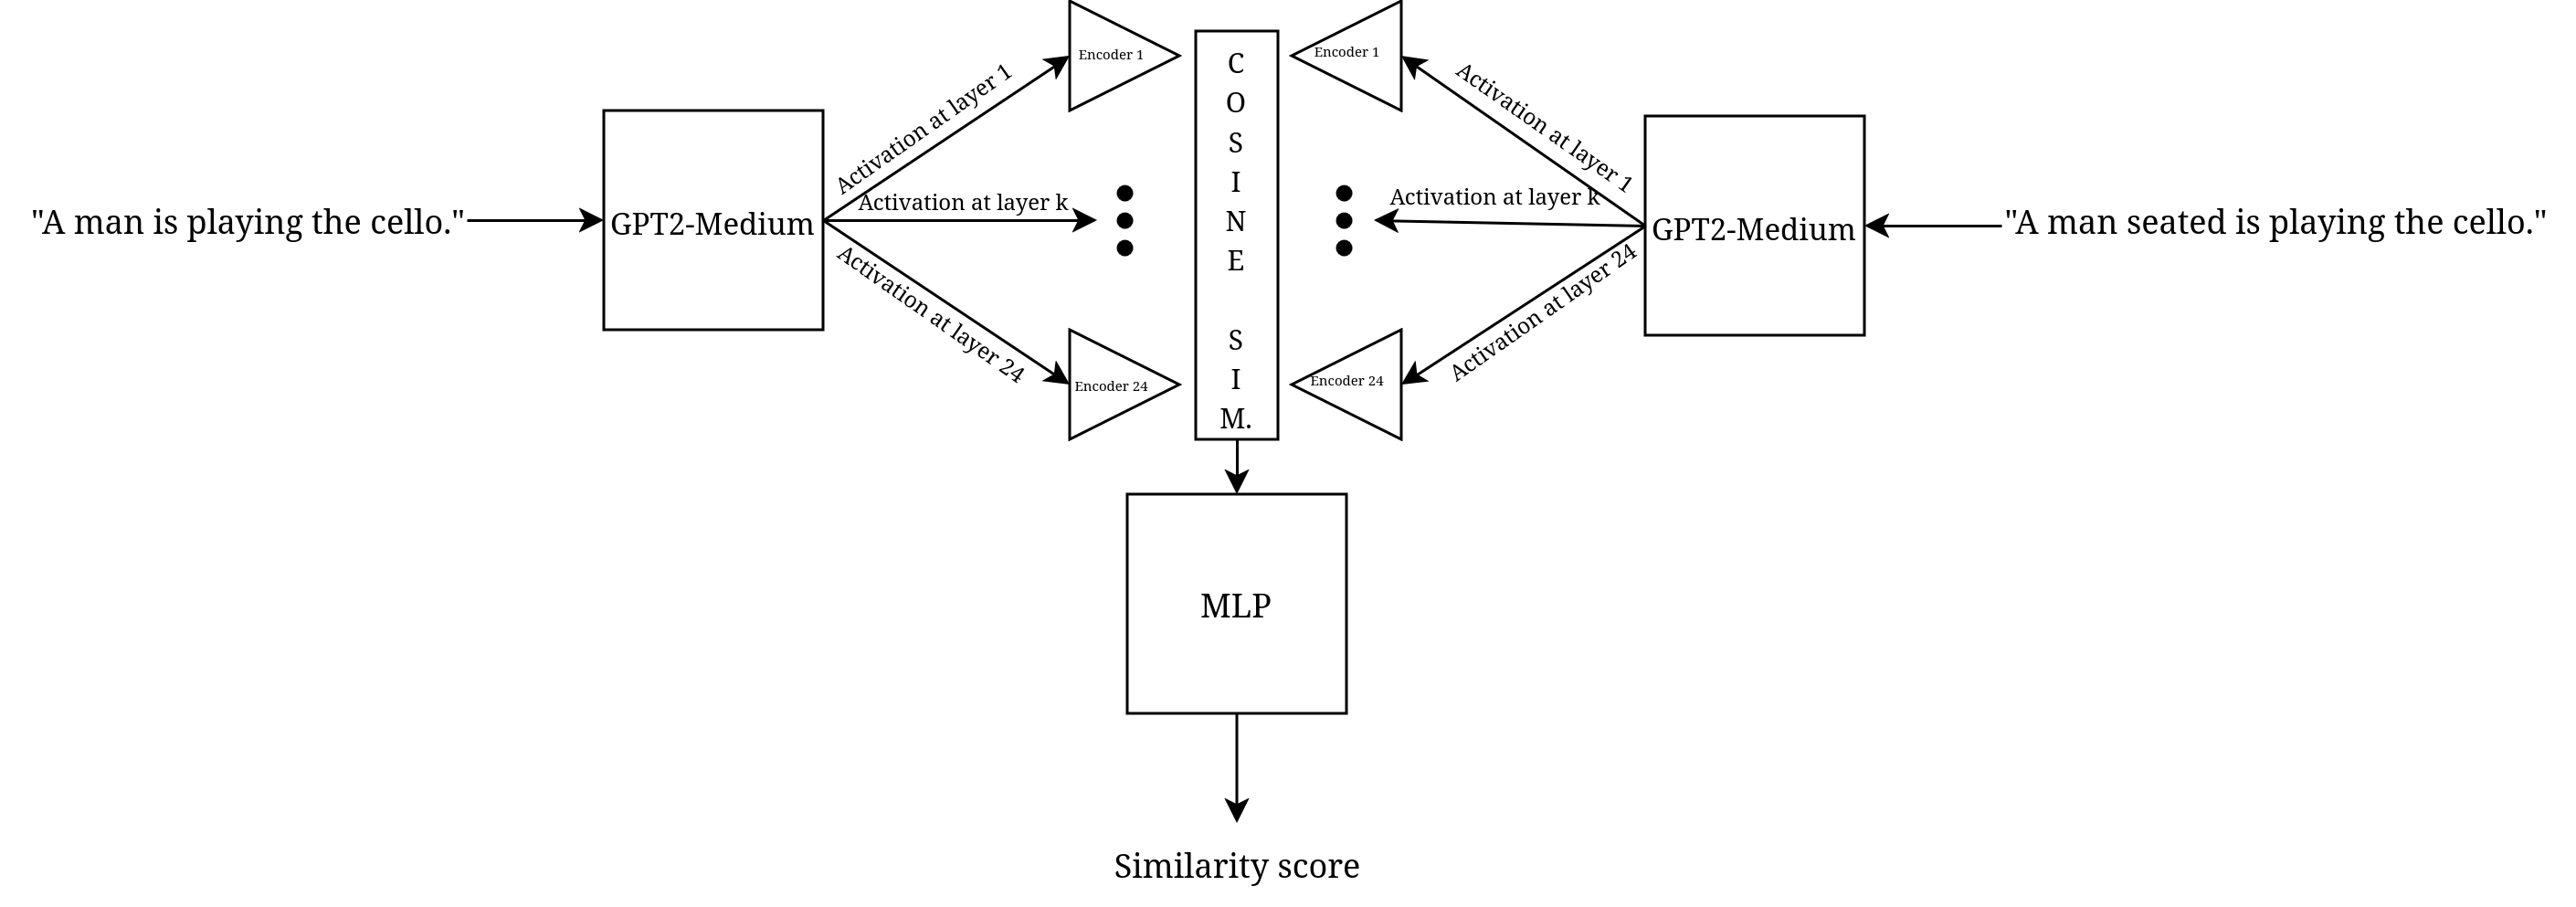
\includegraphics[width=1\linewidth]{model_diagram.png}
%     \caption{Model Diagram}
%     \label{fig:model-diagram}
% \end{figure}

% The architecture we've settled on so far is fairly simple (Figure \ref{fig:model-diagram}). We train an ensemble \footnote{When we say \textit{"ensemble"} here we don't mean it in the traditional sense. Although each of the autoencoders are acting independently, they are joined together after pretraining. They still see independent and different inputs. We had trouble finding a suitable name for this kind of component, so we stuck with \textbf{"ensemble"} even if its not technically correct.} of autoencoders to reconstruct each layer's activations (I.e. twenty-four autoencoders). We pretrain these on twenty-thousand sentence activations generated from the GenericsKB \cite{huggingface:genericskb} dataset. Then, after this pre-training we take the encoder end of each autoencoder and begin STS supervised training. To do this we treat each autoencoder as its own layer-specific Siamese network. We then pass each layer's activation through its respective autoencoder, take the cosine similarity of the two resulant vectors, and collect all twenty-four cosine values into a vector. This is then passed into a simple MLP to do basic pattern recognition on the similarity values.
% \subsection{Insights}
% % Are there any concrete results you can show at this point? How is your model performing compared with expectations?
% Our model is performing \textit{significantly better than expected}. We originally were aiming for roughly \verb|60%| pearson correlation as a stretch goal. Our model achieves a \verb|75.36%| pearson and \verb|73.21%| spearman correlation using our approach. This is nowhere near state of the art, but getting this result takes under two hours of training (On an \verb|RTX3060 12g|) and under four total if we include generating the activations for the pre-training and supervised training beforehand. We are incredibly happy with our performance so far. Moreover we were able to replicate our results (Actually, slightly better at \verb|+~2%| on both pearson and spearman) using \verb|qwen2-0.5b|, a completely different model. The only thing we changed was the input dimension to our autoencoders because \verb|qwen2-0.5b| has a different hidden dimension, otherwise it was a drop-in replacement. This \textit{suggests} that our model would generalize to larger models.

% \subsubsection{Interesting findings}
% \begin{figure}
%     \centering
%     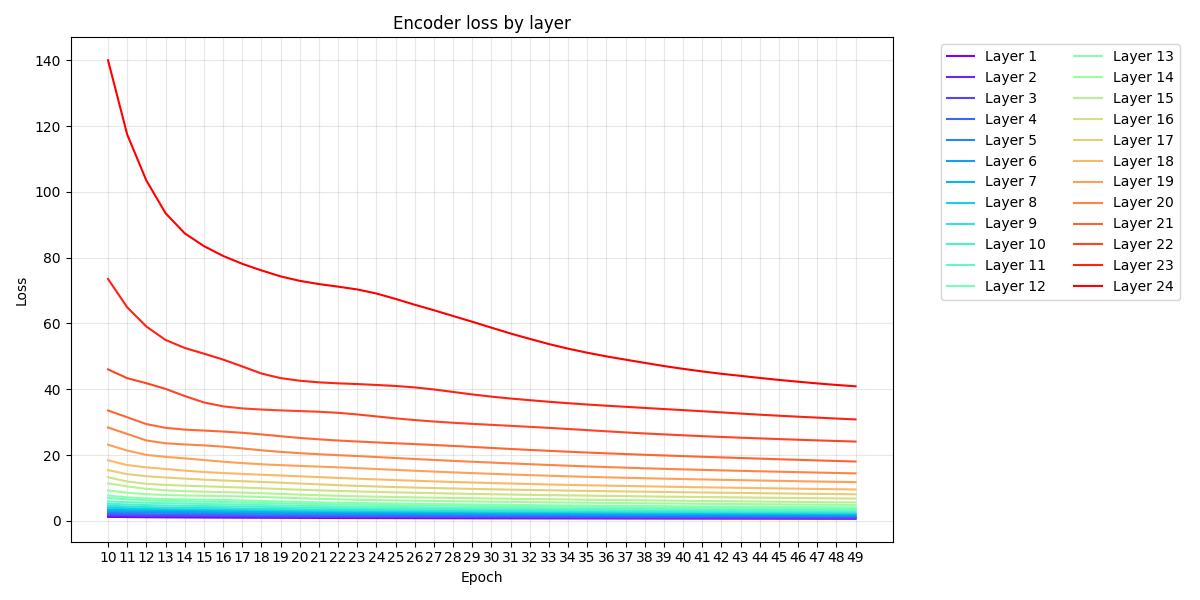
\includegraphics[width=0.85\linewidth]{encoder_loss.png}
%     \caption{Autoencoder loss by layer. $\text{d}_\text{bottleneck} = 256$}
%     \label{fig:autoencoder-loss}
% \end{figure}
% \paragraph{Using autoencoders for pretraining.} We had hit a wall after developing the ensemble of siamese networks approach and performance plateaued for quite a few days at around \verb|60-68%| pearson correlation. We theorized that maybe we can't perform better because we don't have \textit{"enough time"} during supervised training to build good representations. We then thought to try and "pre-train" our siamese networks by first training them as encoders in a set of autoencoders. Our rational for this was that training as an autoencoder would first force the networks to build a good representation of their respective layers before we get anywhere near supervised training. We tried training on \verb|10,000|, \verb|20,000|, and \verb|50,000| sentences from the GenericsKB dataset \cite{huggingface:genericskb} but saw no difference after \verb|20,000|. On the first few training attempts we noticed that performance did not improve at all, even after pre-training. We then graphed each autoencoder's loss over time and got the interesting results of Figure \ref{fig:autoencoder-loss}. This inspired us to increase the bottleneck dimension at the later layers \footnote{For layer i's encoder, $d_\text{bottleneck}(i) = 256 \text{ if } i < 12 \text{ else } 512$}. This brought performance up to where it is now for a gain of roughly \verb|7%|, even though the encoders/pre-trained siamese networks have fewer parameters overall. This suggests that 256 bases is simply not enough to effectively represent the information in the later layers without significant losses, which aligns with our observation that deeper autoencoders didn't help - the issue wasn't architectural complexity but rather the fundamental dimensionality of the bottleneck.\\\\
% We also found that training the autoencoders, even if loss wasn't moving, still had a meaningful effect. We found that up until 250 epochs (About an hour of training) we still saw downstream performance benefits even though reconstruction loss did not significantly improve.

% \paragraph{Accidental reproduction} When producing Figure \ref{fig:autoencoder-loss} we also plotted the average norm and variance of each layer's latent vectors (For the pretraining dataset) and noticed that both quantities increased exponentially with the layer number. We then did some research and found that this is a known result \cite{resid-norm-grows}. It was incredibly satisfying to find out what we had "mined" from our experiments was producing known but still interesting facts about transformers. \\\\
% Intuitively, you'd think this would mean that the loss values we're seeing in Figure \ref{fig:autoencoder-loss} would then not be nearly as bad as they seem. It's $L_2$ reconstruction loss, so if the vector magnitude is higher then you'd expect on average a higher loss even if the \textit{proportion} of reconstruction error is small. Regardless, we could not show any benefits of autoencoder pre-training without increasing the bottleneck size in the later autoencoders. This leads us to believe that the \textit{problem of compression} gets harder, not just the vector magnitude, as the layers go on. This is substantiated by the fact that having a \textit{deeper} autoencoder at later layers (still retaining the bottleneck) \textit{did not improve downstream supervised performance}. Only widening the bottleneck improved performance. This is further evidence that there is a higher quantity of non-redundant information that accumulates as the layers go on in a forward pass of a transformer.

% \paragraph{Ensemble $\stackrel{?}{>}$ Individual} For all of the same reasons that training \textit{all} of the siamese networks together was difficult, so too was training any \textit{particular} siamese network. We found that the best individual siamese network performed with a pearson correlation of \verb|71%|. As you might guess, it was the last one. We haven't had enough time yet to really investigate if our ensemble is better than just taking the last latent, so we won't conclude anything about performance yet but it would not be shocking (nor invalidating) to see that last latent hold all of the information to match the ensemble model. Although we spent most of this project focused on the ensemble model, that was mostly just out of curiosity, not because we had firm convictions that it would be significantly better. We honestly expected the network to ignore more of the layers and just jump right to betting totally on the last one but this wasn't the case. We found that when trying to aggregate the cosine scores, an MLP did the best over something like mean pooling. We expect this is because certain patterns probably appear in the similarity scores that, if learned, give a better picture.\\\\
% Intuitively, though, it might not be obvious that using multiple layer's worth of latents would be more useful than just the last because of the residual connection employed in transformer models -- If the information from the last $n$ layers is just getting propogated anyway, why bother using them independently? We believe that although this is mostly correct, it ignores the findings of Bricken et. al \cite{bricken2023monosemanticity} that demonstrate individual layers having individual responsibilities and "resolving" independent parts of the broader context of a given text input. That's why we believe that multiple layer's embeddings will probably, in the limit, be significantly more useful than just the final layer. Also intuitively, but from a different angle, because a transformer's ultimate goal is token prediction, we could imagine that information in intermediate layers could easily be thrown away because it's not useful for next token prediction, even if it could be useful in another domain -- another reason to consider multiple layer's latents.

% \paragraph{Interesting behavior post supervised training}
% We produced a really interesting graph (Figure \ref{fig:supervised-layer-corr}) wherein after supervised training (I.e. training the model in Figure \ref{fig:model-diagram}), the individual siamese networks did not have the clear increasing correlation with human similarity but instead had a jagged and incredibly nonlinear pattern. We don't really have a good explanation for this but we thought it was cool. Maybe the network is learning to "reuse" some of the less important siamese networks? Maybe its using them to extract really specific information? If it was just ignoring them you'd expect it to do that in the MLP, so we're hesitant to say this is just an artifact of the network learning that particular layers are more important than others.

% \subsection{Challenges}

% % What has been the hardest part of the project you’ve encountered so far?

% \subsubsection{Hyperparameter woes}
% \begin{figure}
%     \centering
%     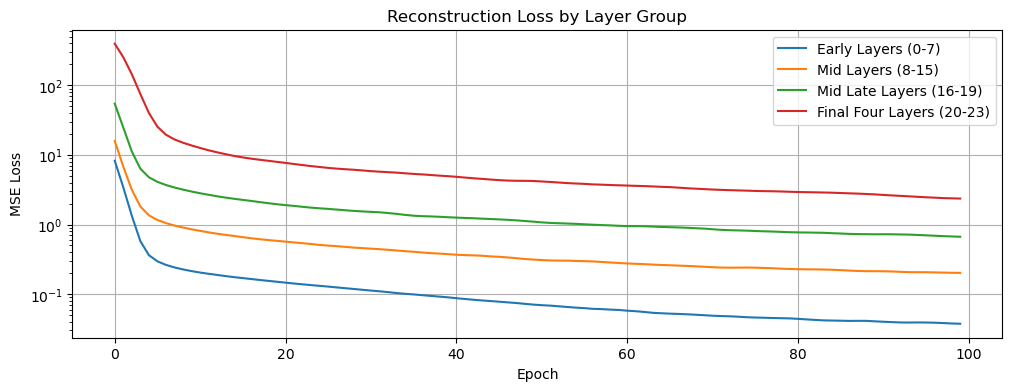
\includegraphics[width=1\linewidth]{final_four_epoch_loss.png}
%     \caption{Loss by layer group over 100 epochs using group-adaptive hidden layer size}
%     \label{fig:epoch_loss}
% \end{figure}
% After seeing the pretraining approach improve performance, we shifted our attention to improving the pretraining reconstruction performance. Our rational was that, at least initially, higher reconstruction performance correlated strongly to higher downstream performance. In order to increase performance, a series of hyperparameter and architecture experiments were conducted. For any given experiment to be considered a potential performance boost, it first needed to decrease the train and test loss by epoch 100 from the baseline autoencoder structure. Once all experiments were conducted, those that passed this check would then be combined and adopted into the autoencoder architecture that then fed into the siamese network, and thus evaluate if "downstream" performance in the form of final train and test correlation was improved based on the changes. The original plan was to perform the experimentation at all layers, however the later layers had the highest loss, so naturally improvements in them would have a greater effect and would be the priority during this experimentation. Furthermore our earlier results suggested that later layers contain significantly higher non-redundant information so the criteria for success was narrowed to improvements in the train and test loss for the final four layers while keeping the structure for other layers the same.
% %Furthermore, the final four layers would have the highest loss and theoretically capture the most complex information, so the criteria for success was narrowed to improvements in the train and test loss for the final four layers while keeping the structure for other layers the same. 
% For the sake of simplicity, of the 24 layers of GPT-2, 0-7 were categorized as early, 8-15 as mid, 16-19 as mid late, and naturally 20-23 as final four. The progression of the baseline train and test loss to beat can be seen in Figure \ref{fig:epoch_loss}, and the final train and test loss values to beat in Table \ref{tab:final_epoch_losses}.
% \begin{table}[h!]
%     \centering
%     \begin{tabular}{|c|c|c|c|}
%     \hline
%     \textbf{Epoch} & \textbf{Phase} & \textbf{Train Loss} & \textbf{Test Loss} \\ \hline
%     \multirow{4}{*}{100} & Early & 0.048 & 1.121 \\ \cline{2-4} 
%      & Mid & 0.260 & 3.492 \\ \cline{2-4} 
%      & Mid Late & 0.847 & 8.891 \\ \cline{2-4} 
%      & Final Four & 2.995 & 18.826 \\ \hline
%     \end{tabular}
%     \caption{Autoencoder losses at Epoch 100 across different phases}
%     \label{tab:final_epoch_losses}
% \end{table}\\
% %%%% NOTE TO HAYDEN. I changed this section a little bit because when training an autoencoder, you need the bottleneck dimension to be less than the original input dimension. The results are the same either way, but I just report where d_bottleneck < d_input
% %
% % First, the number of hidden layers for the final four layers was increased from 256*3 to 256*4 for layer 20, 256*4 to 256*5 for layer 21, 256*4 to 256*6 for layer 22, and 256*4 to 256*7 for layer 23. The rationale behind this was that later layers need more complexity to effectively capture nuances in text similarity, and while enhanced scaling was already occurring a potential enhancement of the scaling could lead to better performance. This experiment saw marginal improvement, so it would be considered a candidate for future adaptation.\\\\
% First, we tried widening the bottleneck dimension in the final four layers from 512 all the way to 768. The rationale behind this was that later layers need more complexity to effectively capture nuances in text similarity, and while enhanced scaling was already occurring a potential enhancement of the scaling could lead to better performance. This experiment saw marginal improvement on the test set, so it would be considered a candidate for future adaptation.\\\\
% Second, the architecture of the encoder and decoder was expanded to include one more activation layer making them deeper. The added depth would provide more parameters and non-linear transformations, which could allow the model to learn more complex mappings and potentially reduce the high reconstruction loss. This experiment saw a significant worsening in performance, and would not be considered a candidate. We believe this is because the added complexity caused the model to overfit on a subset of the distribution.\\\\
% Third, the learning rate for the final four layers would be doubled from baseline. The rationale behind this is that the later layers could have a larger space to traverse to find an optima since their feature space would naturally be more complex. In the baseline model, layer 0 has a learning rate of 3e-4, and each layer afterward is gradually increased by multiplying 3e-4 by 1 + layer number / 24. For example, the final layer would have exactly double the learning rate of the first layer. In this experiment, the scaled learning rates of the final four were doubled. This experiment saw marginal improvement in the train loss and a nonsignificant worsening of test loss, so it would be considered a candidate.\\\\
% Fourth, more dropout layers were introduced in both the encoder and decoder. The rationale behind this was to add more regularization to potentially enhance the generalizability, and hence performance, of the final four layers. However, this experiment saw a dramatic worsening of performance, and would not be considered a candidate. \\\\
% The end results of the experiments can be seen in Table \ref{tab:loss_comparison}.
% \begin{table*}[h!]
%     \centering
%     \begin{tabular}{|l|c|c|c|c|}
%     \hline
%     \textbf{Experiment} & \textbf{Train Loss} & \textbf{\% Difference (Train)} & \textbf{Test Loss} & \textbf{\% Difference (Test)} \\ \hline
%     Baseline & 2.995 & - & 18.826 & - \\ \hline
%     Increased Bottleneck Dimension & 2.377 & {\color{green}-20.64\%} & 18.246 & {\color{green}-3.08\%} \\ \hline
%     Increased Activation Layers & 4.774 & {\color{red}+59.44\%} & 28.300 & {\color{red}+50.33\%} \\ \hline
%     Enhanced Learning Rate & 2.367 & {\color{green}-20.96\%} & 18.840 & {\color{red}+0.07\%} \\ \hline
%     More Dropout & 13.555 & {\color{red}+352.60\%} & 29.610 & {\color{red}+57.27\%} \\ \hline
%     \end{tabular}
%     \caption{Experiment results and differences from the baseline. Loss values are the mean for the final four layers.}
%     \label{tab:loss_comparison}
% \end{table*}\\
% Based on the results, the two candidates that would be incorporated into the autoencoder were increased bottleneck dimension and enhanced learning rate. Once both were incorporated, the autoencoder saw a near 5\% improvement over the baseline and was then used in the siamese network to asses downstream results. In the end, 4 million more parameters were added to the model but \textit{no significant improvement in downstream performance was yielded}. Also, after the end of this experimentation, it was discovered that the original view of the later layers having higher loss was not entirely correct. The magnitude of the vectors produced by increasing layers is simply larger, so the loss appears high but all layers are performing roughly the same in terms of proportional reconstruction loss. However, given that all the layers perform similarly, the conclusions of this experiment are not nullified and can be assumed to apply to all layer groups.\\\\
% Another round of experimentation was performed, but at the normal early, mid, and late layer classifications as opposed to only the final four and with different approaches. But, the same pipeline of needing to beat train and test loss of the baseline autoencoder model, then combining candidates and feeding into the siamese network would be applied. The first was to implement a learning rate scheduler, with the rationale being it would reduce the learning rate over time, preventing the model from overshooting optimal weights, which could be particularly advantageous for later layers. Within PyTorch there are three mainstream options available for learning rate schedulers:
% \begin{itemize}
%     \item \textbf{Exponential Decay (ExponentialLR)}: Gradually reduces the learning rate by a factor after every epoch.
%     \item \textbf{Cosine Annealing (CosineAnnealingLR)}: Reduces the learning rate following a cosine function.
%     \item \textbf{Reduce on Plateau (ReduceLROnPlateau)}: Reduces the learning rate when a metric (e.g., validation loss) stops improving.
% \end{itemize}
% The most simple and logical choice was ReduceLROnPlateau since it was observed that validation loss does not significantly improve past at different epochs depending on the layer. If validation loss did not improve over 20 epochs, i.e. the patience, the learning rate would be reduced by 20\%, and so on until it reached a minimum learning rate of 1e-6. Implementing this scheduler led to no improvement in performance, but cosine annealing was also implemented since the inherent occasional reset of learning rate could benefit the deeper layers. For this scheduler the length of the cosine cycle was 30 epochs, meaning the learning rate would reduce to the minimum, 3e-6 in this case, and then reset to its original value, then decrease again until the max number of epochs was reached. Cosine annealing did not result in improved performance, so neither learning rate schedulers would be considered candidates.\\\\
% Second, a small weight decay term of 1e-4 was added to the optimizer of the similarity learner involved in downstream performance. This does not involve the autoencoder, but the rationale behind this is that the siamese network is clearly overfitting, so by adding regularization to the downstream the test correlation could possibly be improved with less overfitting. However, this led to a 5\% decrease in final test correlation, so this experiment was not incorporated.\\\\
% Third, as another attempt at more regularization in the ensemble, the dropout rate of the autoencoder was increased from .1 to .2. This is different from the previous dropout experiment from the final four testing in that there are the same number of dropout layers in the encoder and decoder, but at each there is more dropout applied. This experiment saw a dramatic worsening of train and test loss across all layers, so the change was not implemented.\\\\
% %%%% NOTE TO HAYDEN. I like this idea but I don't think it's principled enough to be added to our discussion. As is, using KL doesn't really make sense unless we do all the other stuff for VAE's. I think using a VAE is a worthwile avenue to pursue but this is kind of like putting a suit on a baby and wondering why he won't go to work
% %
% % Fourth, the loss function of pure mean squared error was modified to include a Kullback-Leibler (KL) divergence term to make the latent representations close to a normal distribution. The rationale behind this is to take the underlying method powering Variational Autoencoders, KL divergence, and use it here to make latent representations smoother and more generalizable to improve test loss performance. The combined loss function took the following form:
% % \[
% % \text{Loss} = \text{MSE} + 10^{-3} \cdot \text{KL}
% % \]
% % While this idea was nice in theory, in actual application it increased computational complexity severely and made the performance unreliable. As for the final performance, it performed slightly worse than the baseline, so it was not incorporated.\\\\
% Overall, the experimentations performed all resulted in no significant improvement to downstream performance, which was the goal. Given the breadth and depth of the experiments, this could indicate a performance ceiling is being met with the given architecture, and hyperparameter alteration is not the solution to breaking through said ceiling.

% \subsubsection{Attention mechanisms} A natural formulation of our problem is as a set of twenty-four "tokens" that we want to "attend" to to pull out relevant information. We could not find a setup in which this helped our performance in any way. To offer some intuition, attention mechanisms make the assumption that different tokens can be linearly combined in a meaningful way. This \textit{empirically} does not appear to be the case with the latents extracted from \verb|gpt2-medium| suggesting further that different layers have meaningfully different geometries and underlying spaces within their activations (As in Bricken et. al.\cite{bricken2023monosemanticity}).

% \subsubsection{Pooling troubles}
% We tried numerous pooling strategies, none of which worked well. Both at the GPT-2 residual stream token level and at the autoencoder representation level, our attempts at pooling - including approaches similar to those outlined in \cite{tang2024poolingattentioneffectivedesigns} - produced consistently worse results than our layer-wise approach. Simple strategies like mean pooling the latents at each token or combining the twenty-four latents into a single vector all degraded performance.
% \paragraph{Potential future direction} \label{pooling-idea} Another pooling strategy we tried was inspired by the "semantic subspace" idea of Bolukbasi et. al \cite{bolukbasi2016mancomputerprogrammerwoman}. Instead of pooling the latent vectors from GPT-2, we instead pooled the embedding vectors from our encoders. We modified our pretraining approach from the standard bottlenecked autoencoder to a more sophisticated design:
% \begin{enumerate}
%     \item Iteratively project down each latent as normal until it reaches the target bottleneck dimension (No different from normal encoder)
%     \item Project that bottlenecked representation back up to a high dimensional space (E.g. \verb|2048|)
%     \item Sum all of these up-projected vectors (I.e. a sum with twenty-four terms) to produce a single embedding vector. Call this the \textit{total embedding}.
%     \item Now, instead of twenty-four decoders going from the bottleneck dimension up to the input dimension, we instead pass the total embedding to twenty-four separate decoders (I.e. the same vector to twenty-four different encoders)
%     \item Train autoencoders as normal using reconstruction loss
% \end{enumerate}
% The goal of this setup is to learn a \textit{model-wise} representation that reduces redundancy by creating clear semantic subspaces and annihilating duplicate information. Summing is the natural operation here because the model could learn to project different information to different subspaces and keep everything else close to zero.\\\\
% A very naive implementation of this approach produces a single embedding that achieved a \verb|63%| pearson correlation after supervised training - lower than our layerwise approach but significantly better than naive pooling strategies. We believe this direction shows promise for creating unified embeddings, but it would require substantial research effort to fully develop. If given more time, we would have pursued this approach more deeply, as the theoretical elegance of learning orthogonal (or nearly orthogonal) semantic subspaces is particularly appealing.

% \subsubsection{Unsupervised performance}
% Unlike most other models on the leaderboard, our unsupervised performance is \textit{dramatically} worse than its supervised counterpart (\verb|~30-40%| depending on the layer vs \verb|75.36%| supervised. SOTA has closer to a \verb|10-20%| difference). We believe this is because of the autoencoder pre-training approach we took. The autoencoders produce a \textit{compressed} representation, not an especially \textit{spatially related} representation - they are trained to minimize reconstruction loss, not preserve semantic distances. That being said, our supervised performance does eventually do okay, so we're actually optimistic about the quality of the encoded embeddings and believe that although they're not particularly good \textit{as-is} for sentence similarity, they are incredibly rich and useful. This result, while on its face discouraging, is actually something we really want to explore in the future. How is it possible that we can reconstruct a kind of semantic spatiality from otherwise only weakly spatial embeddings? Is it just pattern matching or is it learning to extract complex information from the encoded representation? This gap between supervised and unsupervised performance contributes to our belief that GPT-2's semantic information is encoded in ways that don't naturally align with cosine similarity (or really any simple spatial measure), but can be "disentangled" with appropriate supervision.

% \subsection{Further plans}
% Our further plans are mostly in cleanup, trimming our model down, getting better graphs and building up our less than stellar experiments. We'll also still continue with changing architecture, trying different regularization schemes, etc. We're also currently working on doing hyperparameter sweeps to see if we can squeeze out any extra performance.\\\\
% The last major change we want to try and make is replicating the NLI pretraining approach in the Sentence-BERT \cite{reimers2019sentencebertsentenceembeddingsusing} paper. One thing we've been wrestling with this whole project is overfitting. We're using many, many independent small models trying to solve a hard task -- overfitting generally wins over generalization here. We're incredibly surprised and happy with the results of the autoencoder pretraining and think even more pre-training will only help.\\\\
% Finally, we're considering putting more time and effort into the experiments outlined above  in \ref{pooling-idea} but want to try and maintain a balance between totally new ideas and consolidating what we already have and strengthening our existing results.
% % \verb|TODO| : Consider trying contrastive loss for STS dataset via thresholding or smn. Would need to look at distribution of scores (I think its heavy on the 0's)

% \newpage
% \appendix
% \section{Appendix: Graphs}  % Creates an unnumbered Appendix heading

% \renewcommand{\thefigure}{A.\arabic{figure}}
% \setcounter{figure}{0}  % Reset figure counter to start from 1

% \begin{figure}[!htb]
%     \centering
%     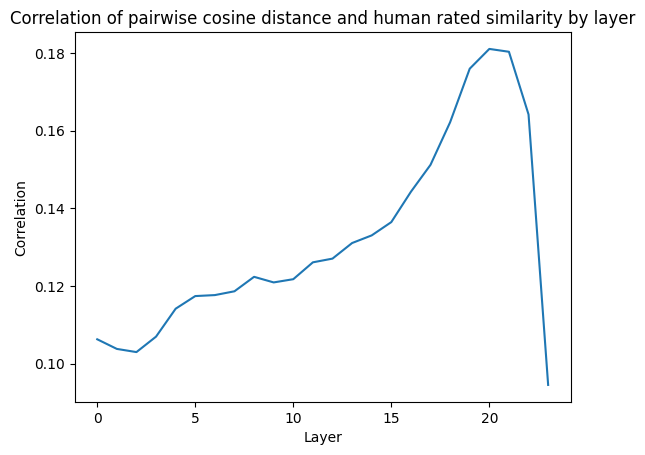
\includegraphics[width=0.57\linewidth]{raw_cosine_sim.png}
%     \caption{Layerwise average correlation between gpt2-medium's embeddings and their cosine similarity vs. human similarity score for the STS training pairs}
%     \label{fig:raw-corr}
% \end{figure}

% \begin{figure}[!htb]
%     \centering
%     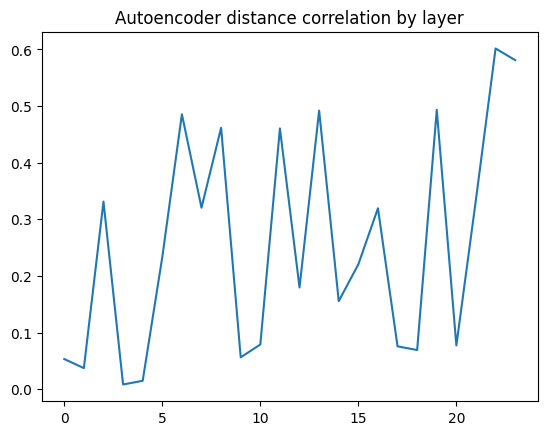
\includegraphics[width=0.5\linewidth]{supervised-layer-corr.png}
%     \caption{Post supervised training encoder embedding cosine distance correlation with human STS score}
%     \label{fig:supervised-layer-corr}
% \end{figure}

\newpage
\bibliography{mybib}{}
\addcontentsline{toc}{section}{References}
\bibliographystyle{plain}
\end{document}
